% Options for packages loaded elsewhere
\PassOptionsToPackage{unicode}{hyperref}
\PassOptionsToPackage{hyphens}{url}
\PassOptionsToPackage{dvipsnames,svgnames,x11names}{xcolor}
%
\documentclass[
  a4paper,
  DIV=11]{scrartcl}

\usepackage{amsmath,amssymb}
\usepackage{iftex}
\ifPDFTeX
  \usepackage[T1]{fontenc}
  \usepackage[utf8]{inputenc}
  \usepackage{textcomp} % provide euro and other symbols
\else % if luatex or xetex
  \usepackage{unicode-math}
  \defaultfontfeatures{Scale=MatchLowercase}
  \defaultfontfeatures[\rmfamily]{Ligatures=TeX,Scale=1}
\fi
\usepackage{lmodern}
\ifPDFTeX\else  
    % xetex/luatex font selection
\fi
% Use upquote if available, for straight quotes in verbatim environments
\IfFileExists{upquote.sty}{\usepackage{upquote}}{}
\IfFileExists{microtype.sty}{% use microtype if available
  \usepackage[]{microtype}
  \UseMicrotypeSet[protrusion]{basicmath} % disable protrusion for tt fonts
}{}
\makeatletter
\@ifundefined{KOMAClassName}{% if non-KOMA class
  \IfFileExists{parskip.sty}{%
    \usepackage{parskip}
  }{% else
    \setlength{\parindent}{0pt}
    \setlength{\parskip}{6pt plus 2pt minus 1pt}}
}{% if KOMA class
  \KOMAoptions{parskip=half}}
\makeatother
\usepackage{xcolor}
\setlength{\emergencystretch}{3em} % prevent overfull lines
\setcounter{secnumdepth}{-\maxdimen} % remove section numbering
% Make \paragraph and \subparagraph free-standing
\ifx\paragraph\undefined\else
  \let\oldparagraph\paragraph
  \renewcommand{\paragraph}[1]{\oldparagraph{#1}\mbox{}}
\fi
\ifx\subparagraph\undefined\else
  \let\oldsubparagraph\subparagraph
  \renewcommand{\subparagraph}[1]{\oldsubparagraph{#1}\mbox{}}
\fi

\usepackage{color}
\usepackage{fancyvrb}
\newcommand{\VerbBar}{|}
\newcommand{\VERB}{\Verb[commandchars=\\\{\}]}
\DefineVerbatimEnvironment{Highlighting}{Verbatim}{commandchars=\\\{\}}
% Add ',fontsize=\small' for more characters per line
\usepackage{framed}
\definecolor{shadecolor}{RGB}{241,243,245}
\newenvironment{Shaded}{\begin{snugshade}}{\end{snugshade}}
\newcommand{\AlertTok}[1]{\textcolor[rgb]{0.68,0.00,0.00}{#1}}
\newcommand{\AnnotationTok}[1]{\textcolor[rgb]{0.37,0.37,0.37}{#1}}
\newcommand{\AttributeTok}[1]{\textcolor[rgb]{0.40,0.45,0.13}{#1}}
\newcommand{\BaseNTok}[1]{\textcolor[rgb]{0.68,0.00,0.00}{#1}}
\newcommand{\BuiltInTok}[1]{\textcolor[rgb]{0.00,0.23,0.31}{#1}}
\newcommand{\CharTok}[1]{\textcolor[rgb]{0.13,0.47,0.30}{#1}}
\newcommand{\CommentTok}[1]{\textcolor[rgb]{0.37,0.37,0.37}{#1}}
\newcommand{\CommentVarTok}[1]{\textcolor[rgb]{0.37,0.37,0.37}{\textit{#1}}}
\newcommand{\ConstantTok}[1]{\textcolor[rgb]{0.56,0.35,0.01}{#1}}
\newcommand{\ControlFlowTok}[1]{\textcolor[rgb]{0.00,0.23,0.31}{#1}}
\newcommand{\DataTypeTok}[1]{\textcolor[rgb]{0.68,0.00,0.00}{#1}}
\newcommand{\DecValTok}[1]{\textcolor[rgb]{0.68,0.00,0.00}{#1}}
\newcommand{\DocumentationTok}[1]{\textcolor[rgb]{0.37,0.37,0.37}{\textit{#1}}}
\newcommand{\ErrorTok}[1]{\textcolor[rgb]{0.68,0.00,0.00}{#1}}
\newcommand{\ExtensionTok}[1]{\textcolor[rgb]{0.00,0.23,0.31}{#1}}
\newcommand{\FloatTok}[1]{\textcolor[rgb]{0.68,0.00,0.00}{#1}}
\newcommand{\FunctionTok}[1]{\textcolor[rgb]{0.28,0.35,0.67}{#1}}
\newcommand{\ImportTok}[1]{\textcolor[rgb]{0.00,0.46,0.62}{#1}}
\newcommand{\InformationTok}[1]{\textcolor[rgb]{0.37,0.37,0.37}{#1}}
\newcommand{\KeywordTok}[1]{\textcolor[rgb]{0.00,0.23,0.31}{#1}}
\newcommand{\NormalTok}[1]{\textcolor[rgb]{0.00,0.23,0.31}{#1}}
\newcommand{\OperatorTok}[1]{\textcolor[rgb]{0.37,0.37,0.37}{#1}}
\newcommand{\OtherTok}[1]{\textcolor[rgb]{0.00,0.23,0.31}{#1}}
\newcommand{\PreprocessorTok}[1]{\textcolor[rgb]{0.68,0.00,0.00}{#1}}
\newcommand{\RegionMarkerTok}[1]{\textcolor[rgb]{0.00,0.23,0.31}{#1}}
\newcommand{\SpecialCharTok}[1]{\textcolor[rgb]{0.37,0.37,0.37}{#1}}
\newcommand{\SpecialStringTok}[1]{\textcolor[rgb]{0.13,0.47,0.30}{#1}}
\newcommand{\StringTok}[1]{\textcolor[rgb]{0.13,0.47,0.30}{#1}}
\newcommand{\VariableTok}[1]{\textcolor[rgb]{0.07,0.07,0.07}{#1}}
\newcommand{\VerbatimStringTok}[1]{\textcolor[rgb]{0.13,0.47,0.30}{#1}}
\newcommand{\WarningTok}[1]{\textcolor[rgb]{0.37,0.37,0.37}{\textit{#1}}}

\providecommand{\tightlist}{%
  \setlength{\itemsep}{0pt}\setlength{\parskip}{0pt}}\usepackage{longtable,booktabs,array}
\usepackage{calc} % for calculating minipage widths
% Correct order of tables after \paragraph or \subparagraph
\usepackage{etoolbox}
\makeatletter
\patchcmd\longtable{\par}{\if@noskipsec\mbox{}\fi\par}{}{}
\makeatother
% Allow footnotes in longtable head/foot
\IfFileExists{footnotehyper.sty}{\usepackage{footnotehyper}}{\usepackage{footnote}}
\makesavenoteenv{longtable}
\usepackage{graphicx}
\makeatletter
\def\maxwidth{\ifdim\Gin@nat@width>\linewidth\linewidth\else\Gin@nat@width\fi}
\def\maxheight{\ifdim\Gin@nat@height>\textheight\textheight\else\Gin@nat@height\fi}
\makeatother
% Scale images if necessary, so that they will not overflow the page
% margins by default, and it is still possible to overwrite the defaults
% using explicit options in \includegraphics[width, height, ...]{}
\setkeys{Gin}{width=\maxwidth,height=\maxheight,keepaspectratio}
% Set default figure placement to htbp
\makeatletter
\def\fps@figure{htbp}
\makeatother

\KOMAoption{captions}{tableheading}
\makeatletter
\makeatother
\makeatletter
\makeatother
\makeatletter
\@ifpackageloaded{caption}{}{\usepackage{caption}}
\AtBeginDocument{%
\ifdefined\contentsname
  \renewcommand*\contentsname{Inhaltsverzeichnis}
\else
  \newcommand\contentsname{Inhaltsverzeichnis}
\fi
\ifdefined\listfigurename
  \renewcommand*\listfigurename{Abbildungsverzeichnis}
\else
  \newcommand\listfigurename{Abbildungsverzeichnis}
\fi
\ifdefined\listtablename
  \renewcommand*\listtablename{Tabellenverzeichnis}
\else
  \newcommand\listtablename{Tabellenverzeichnis}
\fi
\ifdefined\figurename
  \renewcommand*\figurename{Abbildung}
\else
  \newcommand\figurename{Abbildung}
\fi
\ifdefined\tablename
  \renewcommand*\tablename{Tabelle}
\else
  \newcommand\tablename{Tabelle}
\fi
}
\@ifpackageloaded{float}{}{\usepackage{float}}
\floatstyle{ruled}
\@ifundefined{c@chapter}{\newfloat{codelisting}{h}{lop}}{\newfloat{codelisting}{h}{lop}[chapter]}
\floatname{codelisting}{Listing}
\newcommand*\listoflistings{\listof{codelisting}{Listingverzeichnis}}
\makeatother
\makeatletter
\@ifpackageloaded{caption}{}{\usepackage{caption}}
\@ifpackageloaded{subcaption}{}{\usepackage{subcaption}}
\makeatother
\makeatletter
\@ifpackageloaded{tcolorbox}{}{\usepackage[skins,breakable]{tcolorbox}}
\makeatother
\makeatletter
\@ifundefined{shadecolor}{\definecolor{shadecolor}{rgb}{.97, .97, .97}}
\makeatother
\makeatletter
\makeatother
\makeatletter
\makeatother
\ifLuaTeX
\usepackage[bidi=basic]{babel}
\else
\usepackage[bidi=default]{babel}
\fi
\babelprovide[main,import]{ngerman}
% get rid of language-specific shorthands (see #6817):
\let\LanguageShortHands\languageshorthands
\def\languageshorthands#1{}
\ifLuaTeX
  \usepackage{selnolig}  % disable illegal ligatures
\fi
\IfFileExists{bookmark.sty}{\usepackage{bookmark}}{\usepackage{hyperref}}
\IfFileExists{xurl.sty}{\usepackage{xurl}}{} % add URL line breaks if available
\urlstyle{same} % disable monospaced font for URLs
\hypersetup{
  pdftitle={Modellierung der Kaltmiete},
  pdfauthor={Henrik Popp, Kai Herbst, Manuel Zeh},
  pdflang={de},
  colorlinks=true,
  linkcolor={blue},
  filecolor={Maroon},
  citecolor={Blue},
  urlcolor={Blue},
  pdfcreator={LaTeX via pandoc}}

\title{Modellierung der Kaltmiete}
\usepackage{etoolbox}
\makeatletter
\providecommand{\subtitle}[1]{% add subtitle to \maketitle
  \apptocmd{\@title}{\par {\large #1 \par}}{}{}
}
\makeatother
\subtitle{Vergleich Frankfurt am Main und Leipzig}
\author{Henrik Popp, Kai Herbst, Manuel Zeh}
\date{2024-01-31}

\begin{document}
\maketitle
\ifdefined\Shaded\renewenvironment{Shaded}{\begin{tcolorbox}[breakable, frame hidden, sharp corners, boxrule=0pt, borderline west={3pt}{0pt}{shadecolor}, enhanced, interior hidden]}{\end{tcolorbox}}\fi

\renewcommand*\contentsname{Inhaltsverzeichnis}
{
\hypersetup{linkcolor=}
\setcounter{tocdepth}{3}
\tableofcontents
}
\hypertarget{aufgabenstellung}{%
\section{Aufgabenstellung}\label{aufgabenstellung}}

\begin{longtable}[]{@{}
  >{\raggedright\arraybackslash}p{(\columnwidth - 6\tabcolsep) * \real{0.1786}}
  >{\raggedright\arraybackslash}p{(\columnwidth - 6\tabcolsep) * \real{0.6143}}
  >{\raggedright\arraybackslash}p{(\columnwidth - 6\tabcolsep) * \real{0.1357}}
  >{\raggedright\arraybackslash}p{(\columnwidth - 6\tabcolsep) * \real{0.0714}}@{}}
\toprule\noalign{}
\begin{minipage}[b]{\linewidth}\raggedright
Abschnitt
\end{minipage} & \begin{minipage}[b]{\linewidth}\raggedright
Aufgabe
\end{minipage} & \begin{minipage}[b]{\linewidth}\raggedright
Reiner Textumfang
\end{minipage} & \begin{minipage}[b]{\linewidth}\raggedright
Erledigt
\end{minipage} \\
\midrule\noalign{}
\endhead
\bottomrule\noalign{}
\endlastfoot
Einleitung & Auf inhaltliche Aufgabenstellung eingehen & 0,5 - 1 Seiten
& {[}✔{]} \\
Datenerhebung & Wie wurden die Daten erhoben? (Suchfilter, Sortierung) &
1 - 3 Sätze & {[}✔{]} \\
Explorative Datenanalyse & Analyse + eventl. Datenvorverarbeitung & 1 -
2 Seiten & {[} {]} \\
Modellierung & Modellierung + Interpretation & 1 - 2 Seiten. & {[}
{]} \\
Zusammenfassung & Gemeinsam kurz zentrale Ergebnisse zusammenfassen +
Auf Grenzen der Analyse eingehen & 0,5 - 1 Seiten. & {[} {]} \\
\end{longtable}

\begin{itemize}
\tightlist
\item
  Hier auch noch Literatur recherchieren:

  \begin{itemize}
  \tightlist
  \item
    https://de.statista.com/statistik/daten/studie/258635/umfrage/bruttokaltmiete-bewohnter-wohnungen-in-deutschland-nach-bundeslaendern/
  \item
    https://www.deutschlandatlas.bund.de/DE/Karten/Wie-wir-wohnen/040-Mieten.html\#\_6a54aw429
  \item
    https://www.ncbi.nlm.nih.gov/pmc/articles/PMC8053893/
  \item
    https://de.statista.com/statistik/daten/studie/262508/umfrage/mietpreise-in-frankfurt-am-main/
  \item
    https://de.statista.com/statistik/daten/studie/1312743/umfrage/mieten-in-leipzig-nach-dem-baualter-der-wohnung/
  \item
    https://de.statista.com/statistik/daten/studie/535299/umfrage/mietpreise-auf-dem-wohnungsmarkt-in-leipzig/
  \item
    https://de.statista.com/statistik/daten/studie/1312730/umfrage/entwicklung-der-angebotsmieten-in-leipzig/
  \item
    https://link.springer.com/chapter/10.1007/978-3-658-11757-3\_4
  \item
    https://www.ifo.de/DocDL/ifoDD\_14-06\_03-10.pdf
  \end{itemize}
\end{itemize}

\hypertarget{einleitung}{%
\section{Einleitung}\label{einleitung}}

In dieser Fallstudie sollen die Kaltmieten der beiden Städte Frankfurt
am Main und Leipzig miteinander verglichen und modelliert werden. Ziel
ist es, die verschiedenen möglichen Einflussfaktoren auf die Kaltmiete
in den jeweiligen Städte zu bestimmen und eine Modellierung der
Kaltmiete zu erstellen.

Zu Beginn wird auf die Datenerhebung eingegangen. Hier soll erklärt
werden, woher die verarbeiteten Daten stammen und unter welchen
Bedingungen die Daten erhoben wurden. Mit der explorativen Datenanalyse
sollen dann die erhobenen Daten beschrieben und veranschaulicht werden.
Hierbei wird die Vorverarbeitung der Daten beschrieben, im Anschluss
wird mithilfe von Grafiken und dazugehörigen Interpretationen eine
Datenanalyse erstellt. Dabei soll unter anderem herausgefunden werden,
welche erhobenen Variablen den größten Einfluss auf die Kaltmiete einer
Stadt haben oder wie hoch die eventuellen Unterschiede der Mieten in den
beiden Städten sind. Den zentralen Teil des Dokuments stellt die
Modellierung dar. Hier soll die Kaltmiete modelliert, also durch ein
selbsterstelltes statistisches Modell dargestellt werden. Zudem wird das
Modell interpretiert. Zum Abschluss werden die Ergebnisse in der
Zusammenfassung aufgearbeitet und präsentiert.

\hypertarget{datenerhebung}{%
\section{Datenerhebung}\label{datenerhebung}}

Die Datenerhebung fand ausschließlich über den Online-Marktplatz für
Wohnungen und Häuser
\emph{\href{https://www.immobilienscout24.de/}{ImmobilienScout24}}
statt. Die untersuchten Objekte wurden dabei auf den Immobilientyp
\emph{Wohnung} beschränkt, was als Suchkriterium in der Suchleiste des
Portals eingestellt werden kann. Weitere Suchkriterien haben sich auf
den \emph{Ort}, in diesem Fall Frankfurt am Main und Leipzig, und auf
den Objekttyp, hier \emph{Mieten}, beschränkt. Weitere Kriterien wie
\emph{Anzahl der Zimmer}, \emph{Fläche} oder einem \emph{maximalen
Preis} wurden auf den Standardeinstellungen belassen. Anschließend
wurden je Ort der Reihe nach bis zu 45 Objekte in der von
ImmobilienScout24 generierten Reihenfolge überpüft und in eine
Excel-Datei aufgenommen, die im Folgendem als Basis für die Auswertung
dient.

Aufgenommen in die Datenbasis wurden dabei die folgenden Variablen: der
\emph{Ort}, die \emph{Kaltmiete} in Euro, die \emph{Wohnfläche} in
Quadratmetern, das Angebot eines \emph{Parkplatz}, die \emph{Etage},
Anzahl der \emph{Zimmer}, Vorhandensein eines \emph{Balkon}, das
\emph{Baujahr} des Objektes, sowie der entsprechende Link zur Anzeige
und dessen Abrufdatum.

Für die nachfolgenden Auswertungen und Analysen lesen wir zunächst die
Excel-Datei ein:

\begin{Shaded}
\begin{Highlighting}[]
\CommentTok{\# Pfad zur Excel{-}Datei erstellen}
\NormalTok{pfad\_mieten }\OtherTok{\textless{}{-}} \FunctionTok{here}\NormalTok{(}\StringTok{"Mieten.xlsx"}\NormalTok{)}
\CommentTok{\# Daten einlesen}
\NormalTok{mieten }\OtherTok{\textless{}{-}} \FunctionTok{read\_excel}\NormalTok{(pfad\_mieten)}
\end{Highlighting}
\end{Shaded}

Über die Ausgabe der ersten sechs Eintrage erhalten wir einen Einblick
in die Daten:

\begin{Shaded}
\begin{Highlighting}[]
\CommentTok{\# Obere 6 Beobachtungen}
\FunctionTok{head}\NormalTok{(mieten)}
\end{Highlighting}
\end{Shaded}

\begin{verbatim}
# A tibble: 6 x 12
  Ort   Kaltmiete Wohnflaeche Parkplatz Etage Zimmer Balkon Einbaukueche Heizung
  <chr>     <dbl>       <dbl> <chr>     <chr>  <dbl> <chr>  <chr>        <chr>  
1 Fran~      1800        70   ja        1          2 ja     ja           Fußbod~
2 Fran~      1500        60   ja        1          1 ja     ja           Zentra~
3 Fran~      2650       146.  ja        1          3 ja     ja           Fußbod~
4 Fran~      1700        94   ja        2          3 nein   ja           Fußbod~
5 Fran~      2000       113.  ja        3          4 ja     ja           Fußbod~
6 Fran~      1700        84.8 ja        3          3 ja     ja           Fußbod~
# i 3 more variables: Baujahr <dbl>, Link <chr>, Abrufdatum <dttm>
\end{verbatim}

\hypertarget{explorative-datenanalyse}{%
\section{Explorative Datenanalyse}\label{explorative-datenanalyse}}

Zu Beginn der explorativen Datenanalyse muss geprüft werden, ob die in
der Datenquelle enthaltenen Daten auf eine bestimmte Art und Weise
vorverarbeitet oder angepasst werden müssen. Hierzu kann zunächt mit
\texttt{str(mieten)} die Struktur des Datensatzes angezeigt werden.

Einschub (kann noch wo anders platziert werden): Um nicht nur den
Gesamtpreis der Kaltmiete zu betrachten wird der Quadratmeterpreis in
den Datensatz mit aufgenommen:

\begin{Shaded}
\begin{Highlighting}[]
\NormalTok{mieten }\OtherTok{\textless{}{-}}\NormalTok{ mieten }\SpecialCharTok{|\textgreater{}}
  \FunctionTok{mutate}\NormalTok{(}\AttributeTok{ppqm =}\NormalTok{ Kaltmiete }\SpecialCharTok{/}\NormalTok{ Wohnflaeche)}
\end{Highlighting}
\end{Shaded}

\begin{Shaded}
\begin{Highlighting}[]
\FunctionTok{str}\NormalTok{(mieten)}
\end{Highlighting}
\end{Shaded}

\begin{verbatim}
tibble [100 x 13] (S3: tbl_df/tbl/data.frame)
 $ Ort         : chr [1:100] "Frankfurt" "Frankfurt" "Frankfurt" "Frankfurt" ...
 $ Kaltmiete   : num [1:100] 1800 1500 2650 1700 2000 1700 1480 2800 1080 2600 ...
 $ Wohnflaeche : num [1:100] 70 60 146 94 113 ...
 $ Parkplatz   : chr [1:100] "ja" "ja" "ja" "ja" ...
 $ Etage       : chr [1:100] "1" "1" "1" "2" ...
 $ Zimmer      : num [1:100] 2 1 3 3 4 3 2 3 2 4 ...
 $ Balkon      : chr [1:100] "ja" "ja" "ja" "nein" ...
 $ Einbaukueche: chr [1:100] "ja" "ja" "ja" "ja" ...
 $ Heizung     : chr [1:100] "Fußbodenheizung" "Zentralheizung" "Fußbodenheizung" "Fußbodenheizung" ...
 $ Baujahr     : num [1:100] 2022 1970 2017 NA 2015 ...
 $ Link        : chr [1:100] "https://www.immobilienscout24.de/expose/136299839?referrer=RESULT_LIST_LISTING&searchId=69ea3df3-e89a-3ab4-867f"| __truncated__ "https://www.immobilienscout24.de/expose/147138109?referrer=RESULT_LIST_LISTING&searchId=69ea3df3-e89a-3ab4-867f"| __truncated__ "https://www.immobilienscout24.de/expose/148020107?referrer=RESULT_LIST_LISTING&searchId=69ea3df3-e89a-3ab4-867f"| __truncated__ "https://www.immobilienscout24.de/expose/148019739?referrer=RESULT_LIST_LISTING&searchId=69ea3df3-e89a-3ab4-867f"| __truncated__ ...
 $ Abrufdatum  : POSIXct[1:100], format: "2023-12-28" "2023-12-28" ...
 $ ppqm        : num [1:100] 25.7 25 18.2 18.1 17.7 ...
\end{verbatim}

\begin{Shaded}
\begin{Highlighting}[]
\NormalTok{miete\_ffm }\OtherTok{\textless{}{-}} \FunctionTok{subset}\NormalTok{(mieten, Ort }\SpecialCharTok{==} \StringTok{"Frankfurt"}\NormalTok{)}
\NormalTok{miete\_lpz }\OtherTok{\textless{}{-}} \FunctionTok{subset}\NormalTok{(mieten, Ort }\SpecialCharTok{==} \StringTok{"Leipzig"}\NormalTok{)}
\end{Highlighting}
\end{Shaded}

Es kann festgestellt werden, dass im Datensatz sowohl kategoriale
nominale Variablen wie \texttt{Heizung} oder \texttt{Zimmer}, als auch
metrische verhältnisskalierte Variablen wie \texttt{Kaltmiete} oder
\texttt{Wohnflaeche} auftreten. Zunächst werden keine Variablen
angepasst bzw. Werte ersetzt, da für die späteren Diagramme die
kategorial nominalen Variablen als Achsenbeschriftung gut verwendet
werden können.

Zuerst soll auf den Zusammenhang von \texttt{Kaltmiete} und
\texttt{Wohnflaeche} geschaut werden, bei zwei metrisch
verhältnisskalierten Variablen bietet sich dafür ein Scatterplot an.

\begin{Shaded}
\begin{Highlighting}[]
\FunctionTok{gf\_point}\NormalTok{(Kaltmiete }\SpecialCharTok{\textasciitilde{}}\NormalTok{ Wohnflaeche, }\AttributeTok{data =}\NormalTok{ mieten)}
\end{Highlighting}
\end{Shaded}

\begin{figure}[H]

{\centering 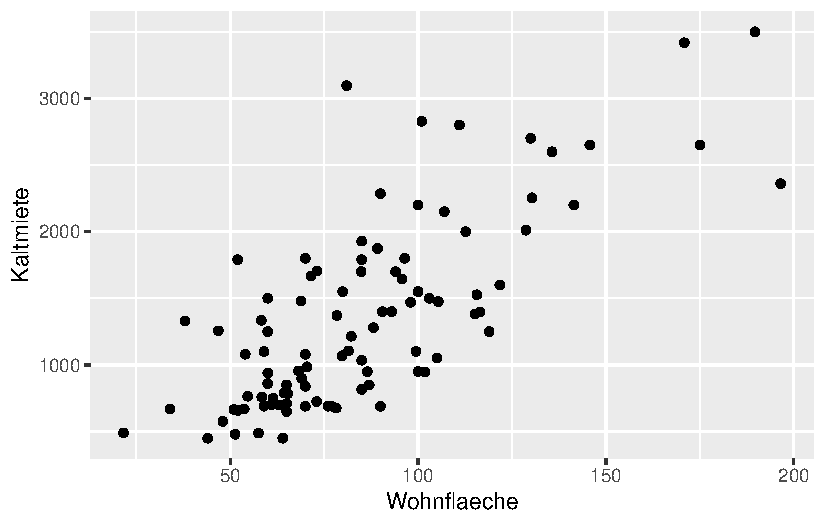
\includegraphics{Mietmodellierung_files/figure-pdf/unnamed-chunk-6-1.pdf}

}

\end{figure}

Grundsätzlich lässt sich ein positiver Zusammenhang zwischen
\texttt{Kaltmiete} und \texttt{Wohnflaeche} erkennen, wobei die Streuung
der Kaltmiete mit zunehmender Wohnfläche zunimmt.

Nun muss dieses Diagramm jedoch um die Information des Ortes erweitert
werden, um eine genauere Aussage treffen zu können. Dafür wird der Code
um den Zusatz \texttt{color\ =\ \textasciitilde{}\ Ort} erweitert:

\begin{Shaded}
\begin{Highlighting}[]
\FunctionTok{gf\_point}\NormalTok{(Kaltmiete }\SpecialCharTok{\textasciitilde{}}\NormalTok{ Wohnflaeche, }\AttributeTok{data =}\NormalTok{ mieten, }\AttributeTok{color =} \SpecialCharTok{\textasciitilde{}}\NormalTok{ Ort)}
\end{Highlighting}
\end{Shaded}

\begin{figure}[H]

{\centering 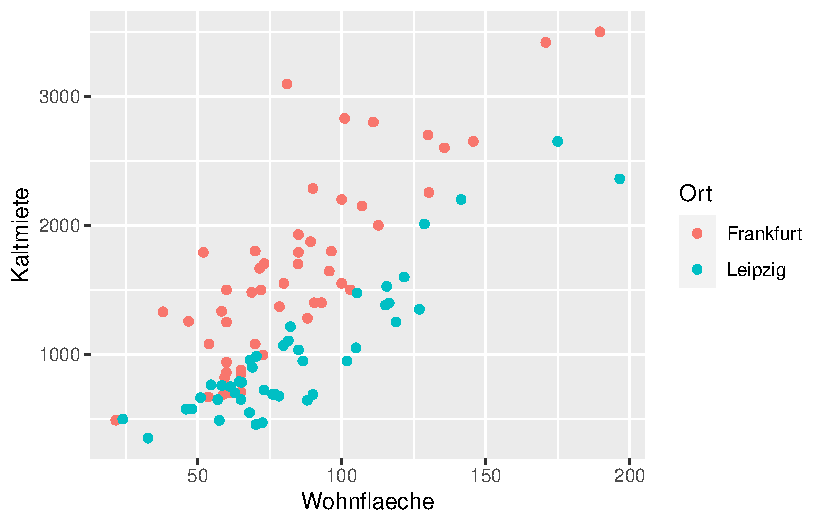
\includegraphics{Mietmodellierung_files/figure-pdf/unnamed-chunk-7-1.pdf}

}

\end{figure}

Hier lässt sich nun erkennen, dass die erfassten Mieten im Datensatz in
Frankfurt tendenziell höher sind, als in Leipzig. Bei vergleichbarer
Wohnfläche liegen die gefärbten Punkte für Frankfurt stets über den
Punkten von Leipzig. Um den Eindruck der Mietunterschiede zu festigen,
kann ein Boxplot verwendet werden.

\begin{Shaded}
\begin{Highlighting}[]
\FunctionTok{gf\_boxplot}\NormalTok{(Kaltmiete }\SpecialCharTok{\textasciitilde{}}\NormalTok{ Ort, }\AttributeTok{data =}\NormalTok{ mieten)}
\end{Highlighting}
\end{Shaded}

\begin{figure}[H]

{\centering 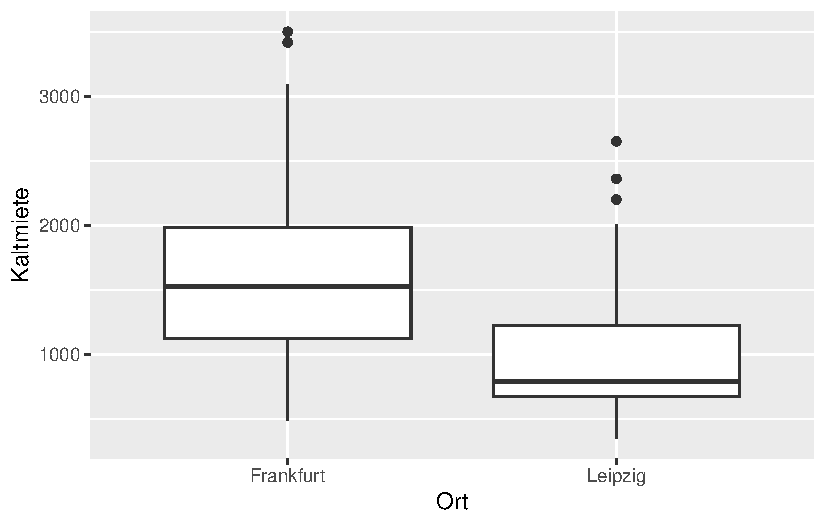
\includegraphics{Mietmodellierung_files/figure-pdf/unnamed-chunk-8-1.pdf}

}

\end{figure}

Das Boxplot zeigt, dass der Median für die Kaltmiete in Frankfurt
deutlich über dem Median von Leipzig liegt. Zudem ist der 1,5-fache
Interquartilsabstand bei Frankfurt größer als bei Leipzig, und die
Whisker sind bei Frankfurt ebenfalls länger. Für Leipzig gibt es jedoch
mehr Ausreißer, nämlich 4, verglichen mit den 2 Ausreißern von
Frankfurt.

Es sollen nun auch die weiteren Variablen untersucht werden, angefangen
mit der Variablen \texttt{Heizung}. Um die verschiedenen Ausprägungen zu
vergleichen und ihre absolute Häufigkeit darzustellen, eignet sich ein
Säulendiagramm:

\begin{Shaded}
\begin{Highlighting}[]
\CommentTok{\# gf\_boxplot(Kaltmiete \textasciitilde{} Heizung, data = mieten, color = \textasciitilde{} Ort)}
\CommentTok{\# gf\_point(Kaltmiete \textasciitilde{} Heizung, data = mieten, color = \textasciitilde{} Ort)}
\FunctionTok{gf\_bar}\NormalTok{( }\SpecialCharTok{\textasciitilde{}}\NormalTok{ Heizung, }\AttributeTok{data =}\NormalTok{ mieten, }\AttributeTok{fill =} \SpecialCharTok{\textasciitilde{}}\NormalTok{ Ort, }\AttributeTok{position =} \FunctionTok{position\_dodge}\NormalTok{()) }\SpecialCharTok{+} \FunctionTok{theme}\NormalTok{(}\AttributeTok{axis.text.x =} \FunctionTok{element\_text}\NormalTok{(}\AttributeTok{angle =} \DecValTok{90}\NormalTok{))}
\end{Highlighting}
\end{Shaded}

\begin{figure}[H]

{\centering 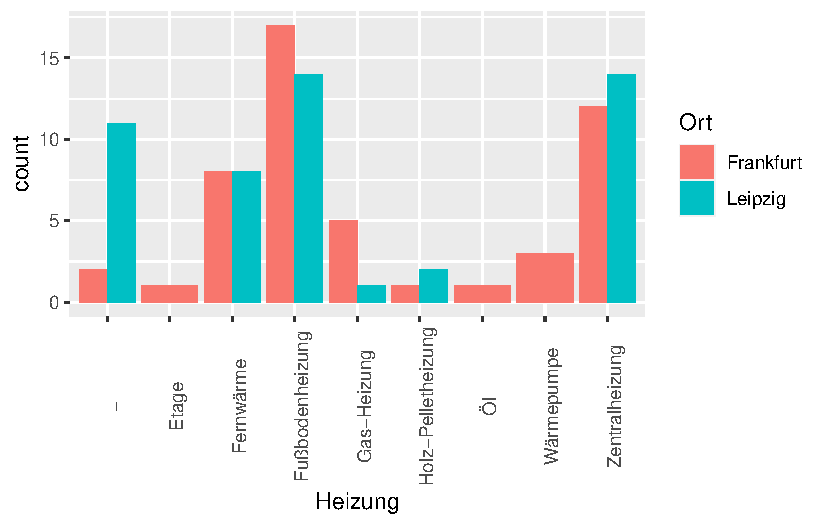
\includegraphics{Mietmodellierung_files/figure-pdf/unnamed-chunk-9-1.pdf}

}

\end{figure}

Das Säulendiagramm zeigt, dass die Fußbodenheizung in Frankfurt am
weitesten verbreitet ist, gefolgt von der Zentralheizung und der
Fernwärme. In Leipzig sind Gas-Heizung und Zentralheizung gleich häufig
vertreten, gefolgt von der Fernwärme. In einigen Beobachtungen und
häufiger in Leipzig als in Frankfurt, wurde der Heizungstyp nicht
angegeben.

Bei der Variablen \texttt{Baujahr} handelt es sich hier um eine diskrete
Variable. Aufgrund der Vielzahl an Jahren im Datensatz eignet sich
jedoch die Verwendung des tatsächlichen Baujahres nicht, da die
Darstellungen sonst sehr unübersichtlich werden. Stattdessen soll eine
Klassifizierung in ``alt - mittel - neu'' vorgenommen werden, um die
Baujahre zusammenzufassen.

\begin{Shaded}
\begin{Highlighting}[]
\NormalTok{mieten }\OtherTok{\textless{}{-}}\NormalTok{ mieten }\SpecialCharTok{\%\textgreater{}\%}
  \FunctionTok{mutate}\NormalTok{(}\AttributeTok{Baujahrgruppe =} \FunctionTok{case\_when}\NormalTok{(}
    \FunctionTok{is.na}\NormalTok{(Baujahr) }\SpecialCharTok{\textasciitilde{}} \StringTok{"NA"}\NormalTok{,}
    \FunctionTok{as.integer}\NormalTok{(Baujahr) }\SpecialCharTok{\textless{}} \DecValTok{1970} \SpecialCharTok{\textasciitilde{}} \StringTok{"alt"}\NormalTok{,}
    \FunctionTok{between}\NormalTok{(}\FunctionTok{as.integer}\NormalTok{(Baujahr), }\DecValTok{1970}\NormalTok{, }\DecValTok{2000}\NormalTok{) }\SpecialCharTok{\textasciitilde{}} \StringTok{"mittel"}\NormalTok{,}
    \ConstantTok{TRUE} \SpecialCharTok{\textasciitilde{}} \StringTok{"neu"}
\NormalTok{  ))}

\FunctionTok{gf\_bar}\NormalTok{( }\SpecialCharTok{\textasciitilde{}}\NormalTok{ Baujahrgruppe, }\AttributeTok{data =}\NormalTok{ mieten, }\AttributeTok{fill =} \SpecialCharTok{\textasciitilde{}}\NormalTok{ Ort, }\AttributeTok{position =} \FunctionTok{position\_dodge}\NormalTok{())}
\end{Highlighting}
\end{Shaded}

\begin{figure}[H]

{\centering 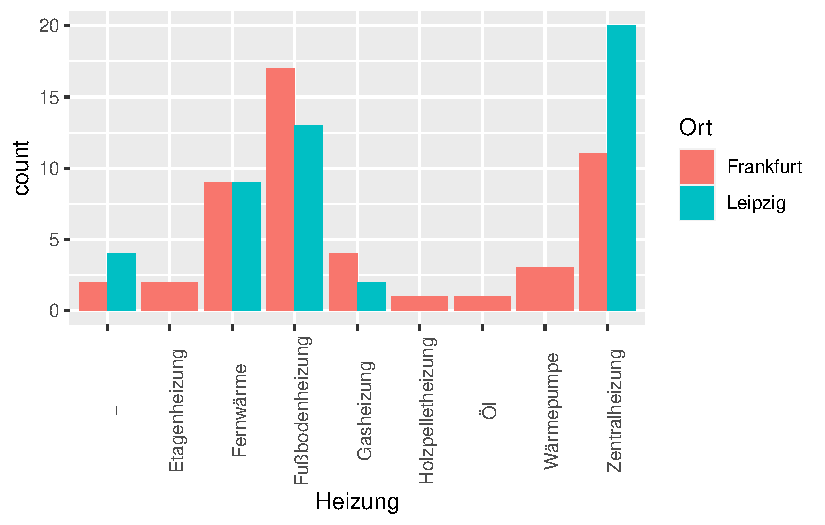
\includegraphics{Mietmodellierung_files/figure-pdf/unnamed-chunk-10-1.pdf}

}

\end{figure}

Im Säulendiagramm ist erkennbar, dass die meisten Beobachtungen in
Frankfurt in die Kategorie ``neu'' (Baujahr \textgreater{} 2000) fallen,
gefolgt von ``alt'' (Baujahr \textless{} 1970) und ``mittel''. In
Leipzig dominieren die Beobachtungen mit ``alt'', dann kommen ``neue''
Baujahre. Es treten in beiden Städten nur wenige Beobachtungen mit
Baujahren zwischen 1970 und 2000 auf, in Leipzig wurde das Baujahr
häufiger nicht angegeben.

\begin{Shaded}
\begin{Highlighting}[]
\FunctionTok{gf\_point}\NormalTok{(Kaltmiete }\SpecialCharTok{\textasciitilde{}}\NormalTok{ Wohnflaeche, }\AttributeTok{data =}\NormalTok{ mieten, }\AttributeTok{color =} \SpecialCharTok{\textasciitilde{}}\NormalTok{ Heizung)}
\end{Highlighting}
\end{Shaded}

\begin{figure}[H]

{\centering 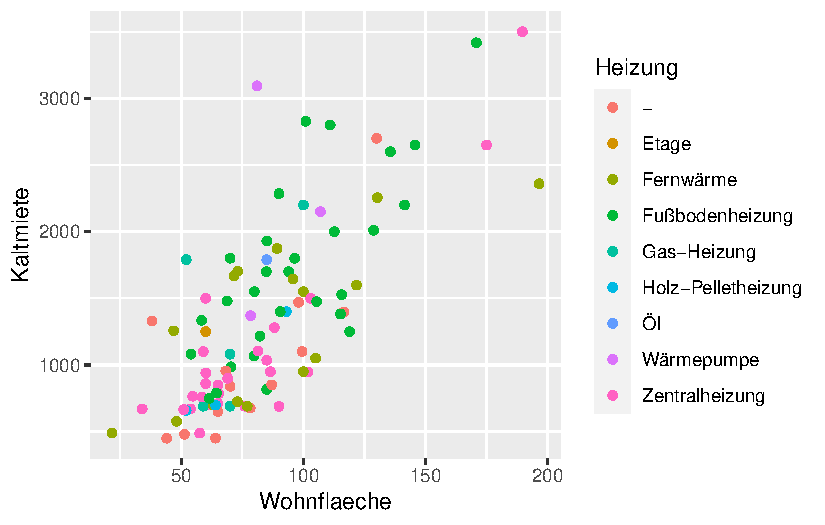
\includegraphics{Mietmodellierung_files/figure-pdf/unnamed-chunk-11-1.pdf}

}

\end{figure}

\begin{Shaded}
\begin{Highlighting}[]
\FunctionTok{gf\_point}\NormalTok{(Kaltmiete }\SpecialCharTok{\textasciitilde{}}\NormalTok{ Wohnflaeche, }\AttributeTok{data =}\NormalTok{ mieten, }\AttributeTok{color =} \SpecialCharTok{\textasciitilde{}}\NormalTok{ Baujahrgruppe)}
\end{Highlighting}
\end{Shaded}

\begin{figure}[H]

{\centering 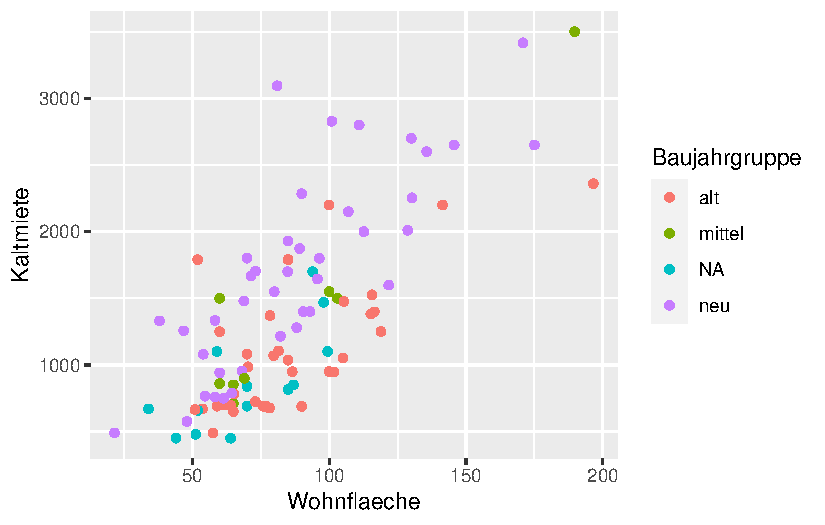
\includegraphics{Mietmodellierung_files/figure-pdf/unnamed-chunk-11-2.pdf}

}

\end{figure}

\begin{Shaded}
\begin{Highlighting}[]
\CommentTok{\# gf\_boxplot(Kaltmiete \textasciitilde{} Einbaukueche, data = mieten, color = \textasciitilde{} Ort)}
\FunctionTok{gf\_boxplot}\NormalTok{(Kaltmiete }\SpecialCharTok{\textasciitilde{}}\NormalTok{ Heizung, }\AttributeTok{data =}\NormalTok{ mieten, }\AttributeTok{color =} \SpecialCharTok{\textasciitilde{}}\NormalTok{ Ort)}
\end{Highlighting}
\end{Shaded}

\begin{figure}[H]

{\centering 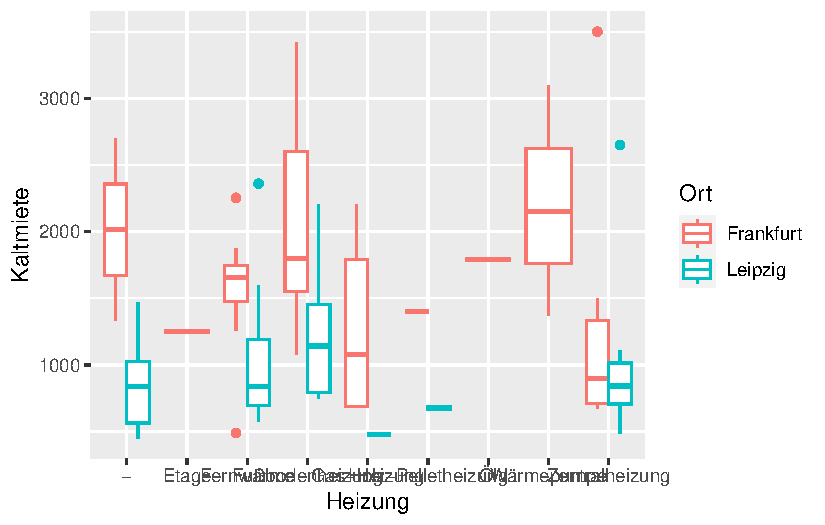
\includegraphics{Mietmodellierung_files/figure-pdf/unnamed-chunk-11-3.pdf}

}

\end{figure}

\begin{Shaded}
\begin{Highlighting}[]
\FunctionTok{gf\_histogram}\NormalTok{(}\SpecialCharTok{\textasciitilde{}}\NormalTok{ Kaltmiete, }\AttributeTok{data =}\NormalTok{ mieten, }\AttributeTok{col =} \SpecialCharTok{\textasciitilde{}}\NormalTok{ Ort, }\AttributeTok{fill =} \SpecialCharTok{\textasciitilde{}}\NormalTok{ Ort)}
\end{Highlighting}
\end{Shaded}

\begin{figure}[H]

{\centering 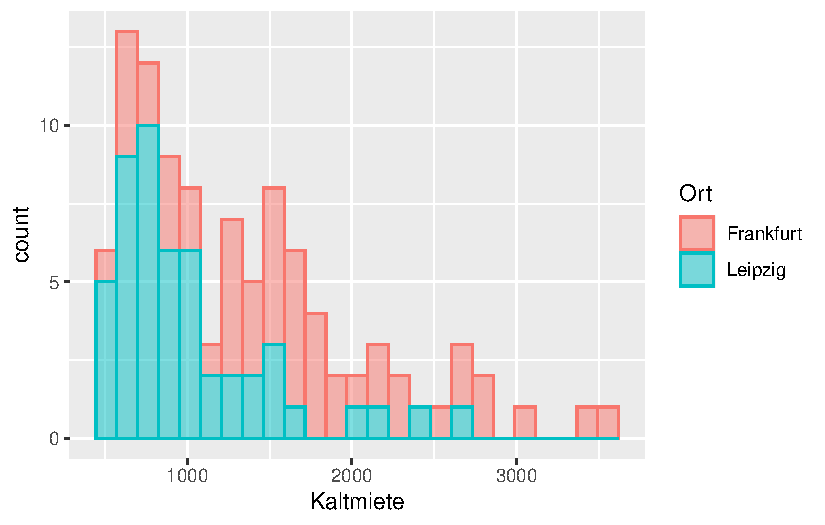
\includegraphics{Mietmodellierung_files/figure-pdf/unnamed-chunk-11-4.pdf}

}

\end{figure}

\begin{Shaded}
\begin{Highlighting}[]
\FunctionTok{mean}\NormalTok{(}\SpecialCharTok{\textasciitilde{}}\NormalTok{ Kaltmiete, }\AttributeTok{data =}\NormalTok{ miete\_ffm)}
\end{Highlighting}
\end{Shaded}

\begin{verbatim}
[1] 1652.121
\end{verbatim}

\begin{Shaded}
\begin{Highlighting}[]
\FunctionTok{mean}\NormalTok{(}\SpecialCharTok{\textasciitilde{}}\NormalTok{ Kaltmiete, }\AttributeTok{data =}\NormalTok{ miete\_lpz)}
\end{Highlighting}
\end{Shaded}

\begin{verbatim}
[1] 1005.372
\end{verbatim}

\#Parkplatz

\begin{Shaded}
\begin{Highlighting}[]
\FunctionTok{gf\_boxplot}\NormalTok{(Kaltmiete }\SpecialCharTok{\textasciitilde{}}\NormalTok{ Parkplatz, }\AttributeTok{data =}\NormalTok{ mieten, }\AttributeTok{color =} \SpecialCharTok{\textasciitilde{}}\NormalTok{ Ort)}
\end{Highlighting}
\end{Shaded}

\begin{figure}[H]

{\centering 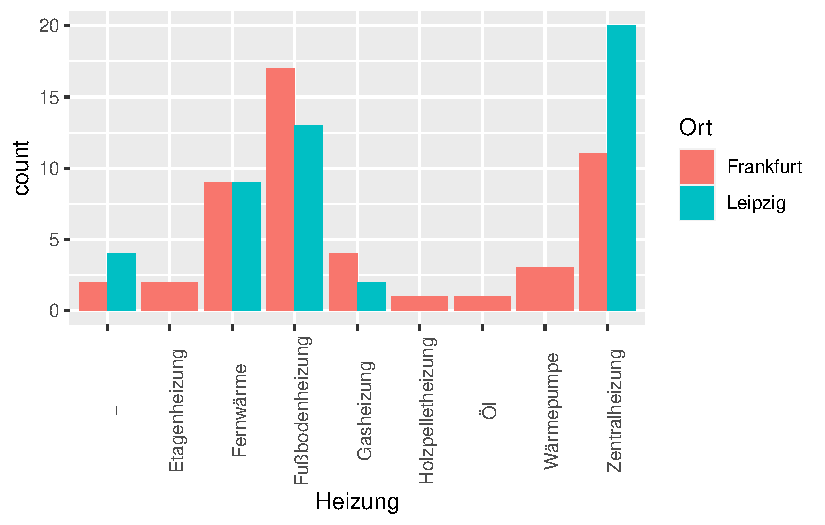
\includegraphics{Mietmodellierung_files/figure-pdf/unnamed-chunk-12-1.pdf}

}

\end{figure}

\begin{Shaded}
\begin{Highlighting}[]
\FunctionTok{tally}\NormalTok{(Ort }\SpecialCharTok{\textasciitilde{}}\NormalTok{ Parkplatz, }\AttributeTok{data =}\NormalTok{ mieten)}
\end{Highlighting}
\end{Shaded}

\begin{verbatim}
           Parkplatz
Ort         ja nein
  Frankfurt 28   22
  Leipzig   20   30
\end{verbatim}

Klare Tendenz in beiden Städten Wohnungen mit Parkplatz sind im Schnitt
teurer ? Parkplatz in der Kaltmiete enthalten? ? Eventuell teurere
Wohnung hat eher eine Tiefgarage oder einen sonstigen Stellplatz auf dem
Grundstück?

\#Balkon

\begin{Shaded}
\begin{Highlighting}[]
\FunctionTok{gf\_boxplot}\NormalTok{(Kaltmiete }\SpecialCharTok{\textasciitilde{}}\NormalTok{ Balkon, }\AttributeTok{data =}\NormalTok{ mieten, }\AttributeTok{color =} \SpecialCharTok{\textasciitilde{}}\NormalTok{ Ort)}
\end{Highlighting}
\end{Shaded}

\begin{figure}[H]

{\centering 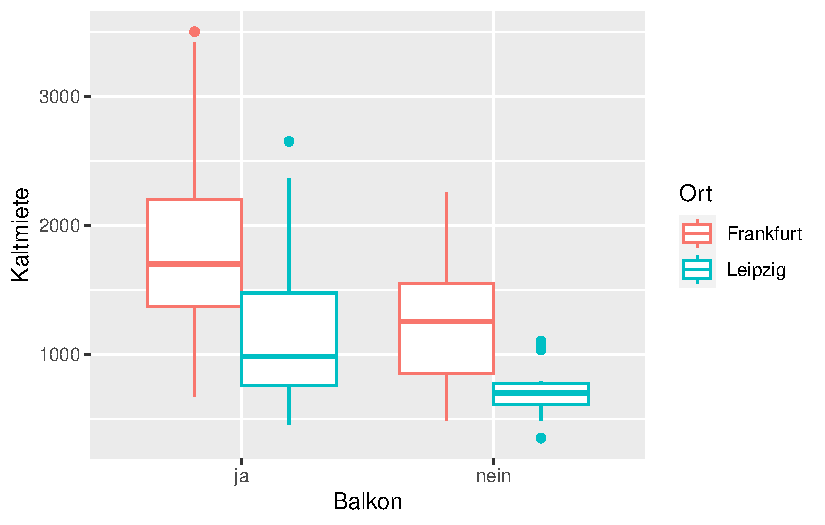
\includegraphics{Mietmodellierung_files/figure-pdf/unnamed-chunk-13-1.pdf}

}

\end{figure}

\begin{Shaded}
\begin{Highlighting}[]
\FunctionTok{gf\_boxplot}\NormalTok{(ppqm }\SpecialCharTok{\textasciitilde{}}\NormalTok{ Balkon, }\AttributeTok{data =}\NormalTok{ mieten, }\AttributeTok{color =} \SpecialCharTok{\textasciitilde{}}\NormalTok{ Ort)}
\end{Highlighting}
\end{Shaded}

\begin{figure}[H]

{\centering 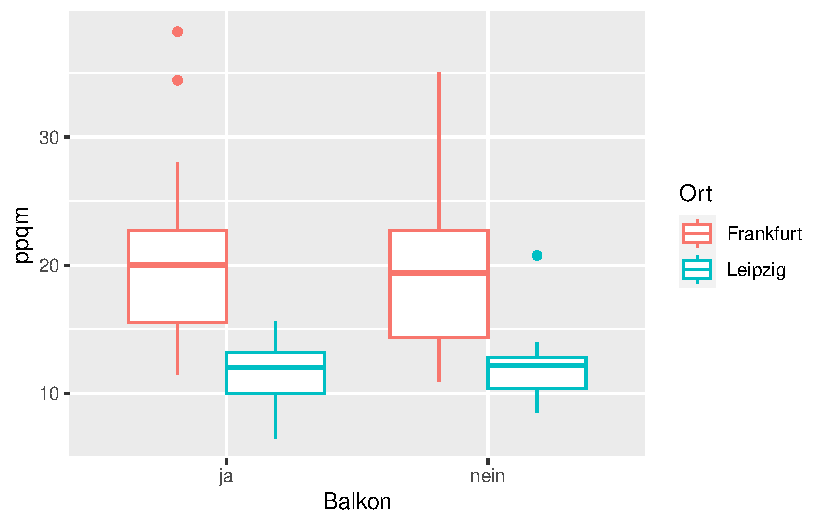
\includegraphics{Mietmodellierung_files/figure-pdf/unnamed-chunk-13-2.pdf}

}

\end{figure}

\begin{Shaded}
\begin{Highlighting}[]
\FunctionTok{tally}\NormalTok{(Ort }\SpecialCharTok{\textasciitilde{}}\NormalTok{ Balkon, }\AttributeTok{data =}\NormalTok{ mieten)}
\end{Highlighting}
\end{Shaded}

\begin{verbatim}
           Balkon
Ort         ja nein
  Frankfurt 35   15
  Leipzig   30   20
\end{verbatim}

Erstes Boxplot zeigt Wohnung mit Balkon sind meist teurer Da der Balkon
auch zu 25\% in die gesamte Wohnflaeche eingerechnet ist, wird im
zweiten Boxplot auch der Quadratmeterpreis betrachtet. Hier ist auch ein
Zusammenhang zwischen Balkon ``Ja'' und einen höheren Kaltmiete zu
erkennen. ?Interpretation: Balkon steigert Kaltmiete unabhängig von der
Wohnfläche. Interessant wäre zusätzlich eine Analyse, wenn Wohnfläcche
um die Fläche des Balkons bereinigt wäre.

\#Zimmer

\begin{Shaded}
\begin{Highlighting}[]
\FunctionTok{gf\_point}\NormalTok{(Kaltmiete }\SpecialCharTok{\textasciitilde{}}\NormalTok{ Zimmer, }\AttributeTok{data =}\NormalTok{ mieten, }\AttributeTok{color =} \SpecialCharTok{\textasciitilde{}}\NormalTok{ Ort)}
\end{Highlighting}
\end{Shaded}

\begin{figure}[H]

{\centering 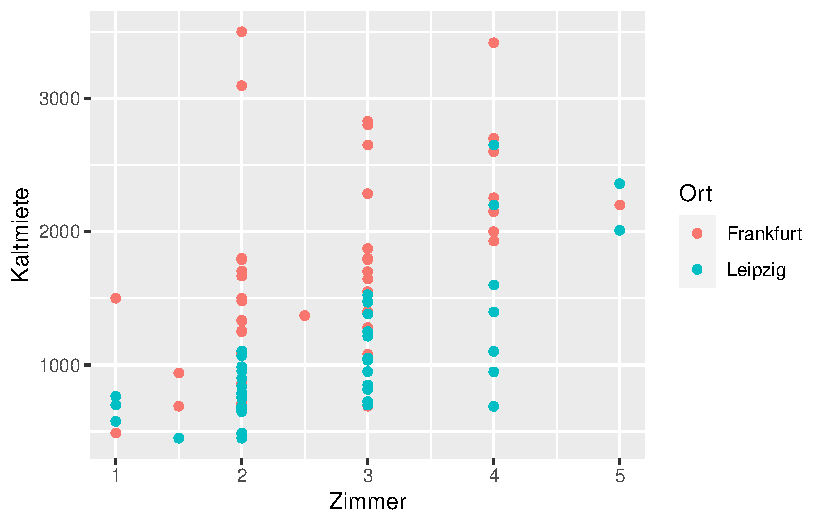
\includegraphics{Mietmodellierung_files/figure-pdf/unnamed-chunk-14-1.pdf}

}

\end{figure}

\begin{Shaded}
\begin{Highlighting}[]
\FunctionTok{gf\_point}\NormalTok{(Wohnflaeche }\SpecialCharTok{\textasciitilde{}}\NormalTok{ Zimmer, }\AttributeTok{data =}\NormalTok{ mieten, }\AttributeTok{color =} \SpecialCharTok{\textasciitilde{}}\NormalTok{ Ort)}
\end{Highlighting}
\end{Shaded}

\begin{figure}[H]

{\centering 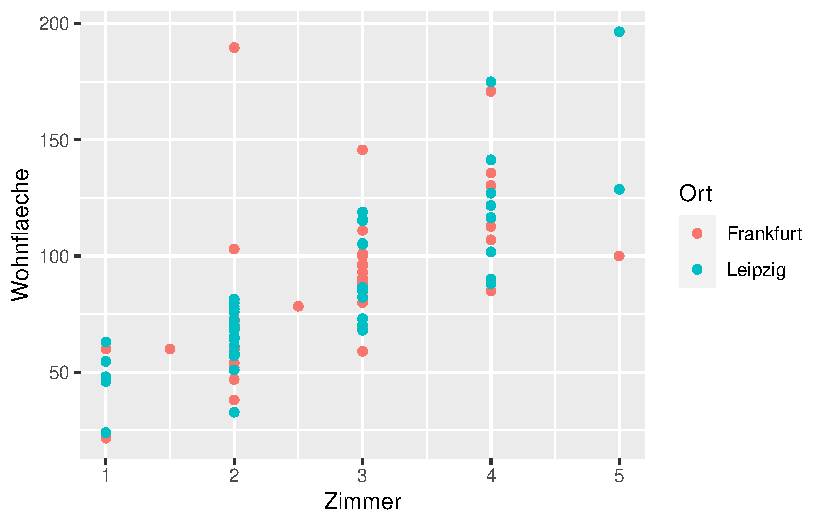
\includegraphics{Mietmodellierung_files/figure-pdf/unnamed-chunk-14-2.pdf}

}

\end{figure}

\begin{Shaded}
\begin{Highlighting}[]
\FunctionTok{gf\_point}\NormalTok{(ppqm }\SpecialCharTok{\textasciitilde{}}\NormalTok{ Zimmer, }\AttributeTok{data =}\NormalTok{ mieten, }\AttributeTok{color =} \SpecialCharTok{\textasciitilde{}}\NormalTok{ Ort)}
\end{Highlighting}
\end{Shaded}

\begin{figure}[H]

{\centering 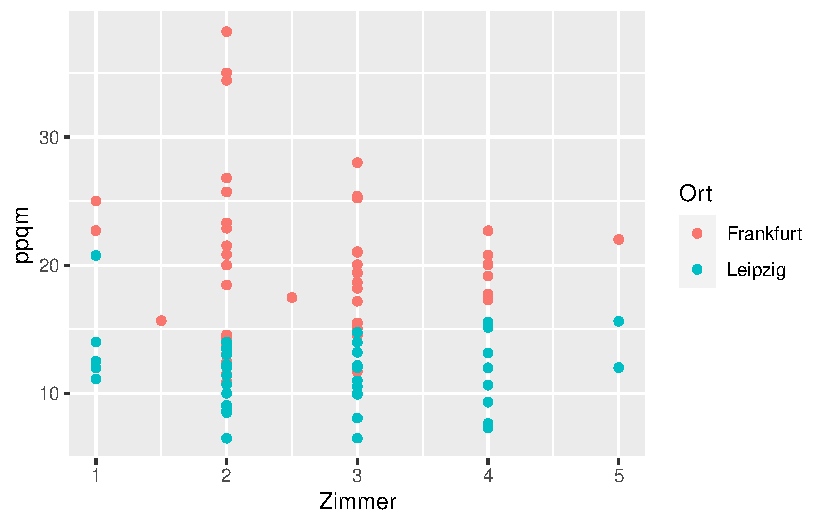
\includegraphics{Mietmodellierung_files/figure-pdf/unnamed-chunk-14-3.pdf}

}

\end{figure}

Insgesamt ist zu erkennen, dass die Variable Zimmer einen Einfluss auf
die Wohnfläche hat. Der Quadratmeterpreis ist bei mehr Zimmern nicht
höher.

\#Etage

\begin{Shaded}
\begin{Highlighting}[]
\FunctionTok{gf\_boxplot}\NormalTok{(Kaltmiete }\SpecialCharTok{\textasciitilde{}}\NormalTok{ Etage, }\AttributeTok{data =}\NormalTok{ mieten)}
\end{Highlighting}
\end{Shaded}

\begin{figure}[H]

{\centering 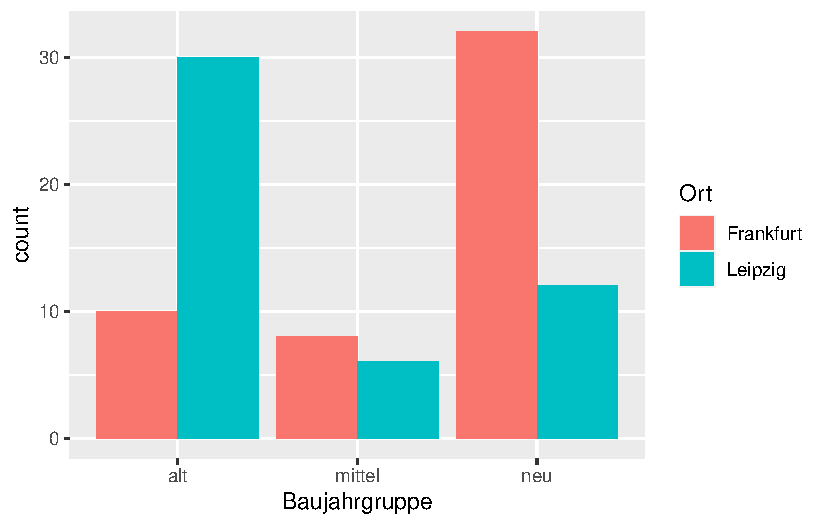
\includegraphics{Mietmodellierung_files/figure-pdf/unnamed-chunk-15-1.pdf}

}

\end{figure}

Schlecht bis gar nicht beschreibbar/interpretierbar

\hypertarget{modellierung}{%
\section{Modellierung}\label{modellierung}}

Aus den zahlreichen Diagrammen des vorherigen Abschnitts der
explorativen Datenanalyse konnten sich bereits diverse Zusammenhänge
erkennen lassen. Dieser letzte Teil der Untersuchung der gegebenen Daten
beschäftigt sich abschließend mit der Modellierung der Kaltmiete unter
Verwendung der zur Verfügung stehenden Variablen wie der Wohnfläche, der
Art der Heizung oder dem Vorhandensein eines Balkons. Ziel ist hierbei
die Erstellung eines Modells, durch das die Variable \texttt{Kaltmiete}
bestmöglich erklärt werden kann.

Das ersten Diagramm der explorativen Datenanalyse, in dem die
\texttt{Kaltmiete} der Inserate zusammen mit deren \texttt{Wohnfläche}
im Streudiagramm dargestellt wurden, lässt einen positiven Zusammenhang
der \texttt{Kaltmiete} zur \texttt{Wohnfläche} vermuten. In einem ersten
einfachen Modell, mit dem dieser Zusammenhang modelliert werden soll,
kann aus den Daten beispielsweise der Durchschnitt des
Quadratmeterpreises berechnet werden.

\begin{Shaded}
\begin{Highlighting}[]
\NormalTok{sum\_wohnflaeche }\OtherTok{\textless{}{-}} \FunctionTok{sum}\NormalTok{(}\SpecialCharTok{\textasciitilde{}}\NormalTok{ Wohnflaeche, }\AttributeTok{data =}\NormalTok{ mieten)}
\NormalTok{sum\_kaltmiete }\OtherTok{\textless{}{-}} \FunctionTok{sum}\NormalTok{(}\SpecialCharTok{\textasciitilde{}}\NormalTok{ Kaltmiete, }\AttributeTok{data =}\NormalTok{ mieten)}
\NormalTok{price\_per\_squaremeter }\OtherTok{\textless{}{-}}\NormalTok{ sum\_kaltmiete }\SpecialCharTok{/}\NormalTok{ sum\_wohnflaeche}
\end{Highlighting}
\end{Shaded}

Damit ergibt sich ersten einfaches Modell für die \texttt{Kaltmiete}
unter Verwendung der \texttt{Wohnfläche} als unabhängige Variable
folgende Gleichung:

\[ Kaltmiete = Wohnfläche \cdot 15.78 € \] Wir betrachten das Modell,
indem die berechnete Gerade in das Streudiagramm der explorativen
Datenanalyse eingezeichnet wird:

\begin{Shaded}
\begin{Highlighting}[]
\NormalTok{pps\_x }\OtherTok{=} \FunctionTok{c}\NormalTok{(}\DecValTok{0}\NormalTok{, }\DecValTok{200}\NormalTok{)}
\NormalTok{pps\_y }\OtherTok{=} \FunctionTok{c}\NormalTok{(}\DecValTok{0}\NormalTok{, price\_per\_squaremeter }\SpecialCharTok{*} \DecValTok{200}\NormalTok{)}
\FunctionTok{gf\_line}\NormalTok{(pps\_y }\SpecialCharTok{\textasciitilde{}}\NormalTok{ pps\_x, }\AttributeTok{color =} \StringTok{"red"}\NormalTok{) }\SpecialCharTok{|\textgreater{}} \FunctionTok{gf\_point}\NormalTok{(Kaltmiete }\SpecialCharTok{\textasciitilde{}}\NormalTok{ Wohnflaeche, }\AttributeTok{data =}\NormalTok{ mieten, }\AttributeTok{color =} \SpecialCharTok{\textasciitilde{}}\NormalTok{ Ort)}
\end{Highlighting}
\end{Shaded}

\begin{figure}[H]

{\centering 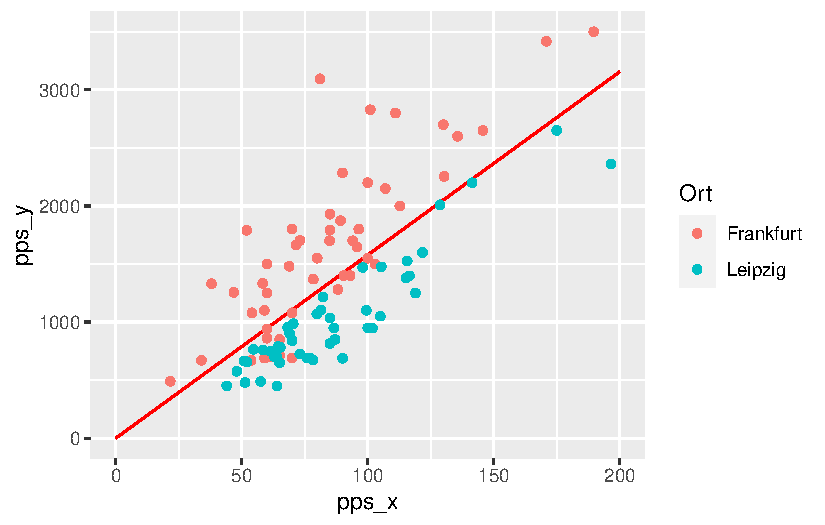
\includegraphics{Mietmodellierung_files/figure-pdf/unnamed-chunk-17-1.pdf}

}

\end{figure}

Dazu kann noch der Korrelationskoeffizient bestimmt werden.

\begin{Shaded}
\begin{Highlighting}[]
\NormalTok{cor\_miete\_flaeche }\OtherTok{=} \FunctionTok{cor}\NormalTok{(Wohnflaeche }\SpecialCharTok{\textasciitilde{}}\NormalTok{ Kaltmiete, }\AttributeTok{data =}\NormalTok{ mieten)}
\end{Highlighting}
\end{Shaded}

Dabei wird festgestellt, dass die \texttt{Kaltmiete} zu 0.7500624\% mit
der Wohnfläche korreliert. Das Modell kann demnach bereits für einen
groben Richtwert verwendet werden. Ziel ist jedoch eine noch genauere
Modellierung der Kaltmiete unter Berücksichtigung der weiteren Daten.

Um die weiteren Variablen miteinzubeziehen, verwenden wir die lineare
Regression, die mit der \texttt{lm()}-Funktion auf die Daten angewendet
werden kann. Wir starten zunächst erneut mit der \texttt{Kaltmiete} und
der \texttt{Wohnflaeche}.

\begin{Shaded}
\begin{Highlighting}[]
\NormalTok{km.lm1 }\OtherTok{\textless{}{-}} \FunctionTok{lm}\NormalTok{(Kaltmiete }\SpecialCharTok{\textasciitilde{}}\NormalTok{ Wohnflaeche, }\AttributeTok{data =}\NormalTok{ mieten)}
\FunctionTok{summary}\NormalTok{(km.lm1)}
\end{Highlighting}
\end{Shaded}

\begin{verbatim}

Call:
lm(formula = Kaltmiete ~ Wohnflaeche, data = mieten)

Residuals:
   Min     1Q Median     3Q    Max 
-819.6 -306.4 -115.6  296.1 1819.5 

Coefficients:
            Estimate Std. Error t value Pr(>|t|)    
(Intercept)  -59.612    132.152  -0.451    0.653    
Wohnflaeche   16.483      1.468  11.227   <2e-16 ***
---
Signif. codes:  0 '***' 0.001 '**' 0.01 '*' 0.05 '.' 0.1 ' ' 1

Residual standard error: 466 on 98 degrees of freedom
Multiple R-squared:  0.5626,    Adjusted R-squared:  0.5581 
F-statistic:   126 on 1 and 98 DF,  p-value: < 2.2e-16
\end{verbatim}

Mit einem Bestimmtheitsmaß von \(R^2 ~ 0.56\), haben wir mit der
linearen Regression allein unter Verwendung der \texttt{Wonflaeche} noch
kein gutes Modell erzeugt.

Da zu Beginn der explorativen Datenanalyse festgestellt wurde, dass die
Kaltmieten zwischen den beiden Orten Frankfurt am Main und Leipzig unter
sonst gleichen Bedingungen unterscheidet, soll diese zuerst in die
Modellierung miteinbezogen werden.

\begin{Shaded}
\begin{Highlighting}[]
\NormalTok{km.lm2 }\OtherTok{\textless{}{-}} \FunctionTok{lm}\NormalTok{(Kaltmiete }\SpecialCharTok{\textasciitilde{}}\NormalTok{ Wohnflaeche }\SpecialCharTok{+}\NormalTok{ Ort, }\AttributeTok{data =}\NormalTok{ mieten)}
\FunctionTok{summary}\NormalTok{(km.lm2)}
\end{Highlighting}
\end{Shaded}

\begin{verbatim}

Call:
lm(formula = Kaltmiete ~ Wohnflaeche + Ort, data = mieten)

Residuals:
   Min     1Q Median     3Q    Max 
-730.6 -192.8   22.2  177.1 1492.2 

Coefficients:
            Estimate Std. Error t value Pr(>|t|)    
(Intercept)  261.025     98.958   2.638  0.00972 ** 
Wohnflaeche   16.565      1.039  15.940  < 2e-16 ***
OrtLeipzig  -655.134     65.978  -9.930  < 2e-16 ***
---
Signif. codes:  0 '***' 0.001 '**' 0.01 '*' 0.05 '.' 0.1 ' ' 1

Residual standard error: 329.9 on 97 degrees of freedom
Multiple R-squared:  0.7831,    Adjusted R-squared:  0.7786 
F-statistic: 175.1 on 2 and 97 DF,  p-value: < 2.2e-16
\end{verbatim}

Durch das Miteinbeziehen des Ortes steigert sich das Bestimmtheitsmaß
bereits auf \(R^2 ~ 0.78\). An der Zusammenfassung der Ergebnisse lässt
sich außerdem ablesen, dass in Leipzig die Kaltmiete im Schnitt 655,13€
billiger als in Leipzig ist. Das Modell lässt sich nun wie folgt
darstellen:

\[ Kaltmiete = 261.03 + Wohnflaeche \cdot 16.57 + \beta1 \cdot -655.13 \]

\hypertarget{rest}{%
\section{Rest}\label{rest}}

Modellieren Sie in diesem Abschnitt die Miete und interpretieren Sie Ihr
Ergebnis.

Bei Einzelarbeiten sollte der reine Text (ohne Code, Abbildungen etc.)
einen Umfang von ca. 0,5--1 Seiten haben, bei Gruppenarbeiten einen von
ca. 1--2 Seiten.

Modell schätzen:

\begin{Shaded}
\begin{Highlighting}[]
\CommentTok{\# Modell\_Mieten \textless{}{-} lm(Kaltmiete \textasciitilde{} 1, data = mieten)}
\CommentTok{\# summary(Modell\_Mieten)}
\end{Highlighting}
\end{Shaded}

Lorem ipsum dolor sit amet, consetetur sadipscing elitr, sed diam nonumy
eirmod tempor invidunt ut labore et dolore magna aliquyam erat, sed diam
voluptua. At vero eos et accusam et justo duo dolores et ea rebum. Stet
clita kasd gubergren, no sea takimata sanctus est Lorem ipsum dolor sit
amet. Lorem ipsum dolor sit amet, consetetur sadipscing elitr, sed diam
nonumy eirmod tempor invidunt ut labore et dolore magna aliquyam erat,
sed diam voluptua. At vero eos et accusam et justo duo dolores et ea
rebum. Stet clita kasd gubergren, no sea takimata sanctus est Lorem
ipsum dolor sit amet.

\hypertarget{zusammenfassung}{%
\section{Zusammenfassung}\label{zusammenfassung}}

Lorem ipsum dolor sit amet, consetetur sadipscing elitr, sed diam nonumy
eirmod tempor invidunt ut labore et dolore magna aliquyam erat, sed diam
voluptua. At vero eos et accusam et justo duo dolores et ea rebum. Stet
clita kasd gubergren, no sea takimata sanctus est Lorem ipsum dolor sit
amet. Lorem ipsum dolor sit amet, consetetur sadipscing elitr, sed diam
nonumy eirmod tempor invidunt ut labore et dolore magna aliquyam erat,
sed diam voluptua. At vero eos et accusam et justo duo dolores et ea
rebum. Stet clita kasd gubergren, no sea takimata sanctus est Lorem
ipsum dolor sit amet.

\begin{center}\rule{0.5\linewidth}{0.5pt}\end{center}

\hypertarget{quellen-und-hilfsmittel}{%
\section{Quellen und Hilfsmittel}\label{quellen-und-hilfsmittel}}

Führen Sie hier die verwendeten Hilfsmittel sowie die verwendete
Literatur auf.



\end{document}
